%!TEX root = ../main.tex

\begin{figure}
%\begin{center}
\tikzset{
triangle/.style = {regular polygon,regular polygon sides=3,draw,inner sep = 2},
circ/.style = {circle,fill=cyan!10,draw,inner sep = 3},
term/.style = {circle,draw,inner sep = 1.5,fill=black},
sq/.style = {rectangle,fill=gray!20, draw, inner sep = 4}
}

\begin{subfigure}{.45\columnwidth}
\centering
\begin{tikzpicture}[scale=0.9]
\tikzstyle{level 1}=[level distance=9mm,sibling distance = 22mm]
\tikzstyle{level 2}=[level distance=7mm,sibling distance=10mm]
\tikzstyle{level 3}=[level distance=7mm,sibling distance=6mm]
\tikzstyle{level 4}=[level distance=7mm,sibling distance=5mm]

%node (ij) is the j th node in i th level

\begin{scope}[->, >=stealth]
\node (0) [circ] {}
child {
  node (00) [triangle] {}
  child {
    node (000) [circ] {}
    child {
      node (0000) [term, label=below:{}] {}
      edge from parent node [left] {\scriptsize $c$}
    }
    child {
      node (0001) [term, label=below:{}] {}
      edge from parent node [right] {\scriptsize $d$}
      }
    edge from parent node [left] {}
  }
  child {
    node (001) [circ] {}
    child {
      node (0010) [term, label=below:{}] {}
      edge from parent node [left] {\scriptsize $c$}
    }
    child {
      node (0011) [term, label=below:{}] {}
      edge from parent node [right] {\scriptsize $d$}
      }
    edge from parent node [right] {} 
  }
  edge from parent node [above] {\scriptsize$a$}
}
child {
  node (01) [triangle] {}
   child {
     node (010) [circ] {}
     child {
      node (0100) [term, label=below:{}] {}
      edge from parent node [left] {\scriptsize $e$}
    }
    child {
      node (0101) [term, label=below:{}] {}
      edge from parent node [right] {\scriptsize $f$}
      }
    edge from parent node [left] {}
  }
  child {
    node (011) [circ] {}
    child {
      node (0110) [term, label=below:{}] {}
      edge from parent node [left] {\scriptsize $e$}
    }
    child {
      node (0111) [term, label=below:{}] {}
      edge from parent node [right] {\scriptsize $f$}
      }
    edge from parent node [right] {} 
  }
  edge from parent node [above] {\scriptsize$b$}
}
;
\end{scope}

%observations
%\draw [dashed, thick, red, in=150,out=30](00) to (01) ;

  \node[fit=(0),dashed,thick,red, draw, circle,inner sep=1pt] {};
\draw [dashed, thick, blue, in=150,out=30] (000) to (001) ;
\draw [dashed, thick, ForestGreen, in=150,out=30] (010) to (011);

%node labels
\node [black] at (0,0.35) {\scriptsize $r$};
\node [black] at (-1,-0.55) {\scriptsize $u_1$};
\node [black] at (1, -0.55) {\scriptsize $u_2$};
\node [black] at (-2, -1.5) {\scriptsize $u_3$};
\node [black] at (-.25, -1.5) {\scriptsize $u_4$};

\node [black] at (0.25, -1.5) {\scriptsize $u_5$};
\node [black] at (2, -1.5) {\scriptsize $u_6$};

%obs labels
\node [red] at (0,-.5) {\scriptsize $I_1$};
\node [blue] at (-1.1,-1.6) {\scriptsize $I_2$};
\node [ForestGreen] at (1.1,-1.6) {\scriptsize $I_3$};



\end{tikzpicture}

\caption{$\Max$ with perfect recall}
\label{fig-allexmp-pftrec}
\end{subfigure}
\quad
\begin{subfigure}{.45\columnwidth}
\centering
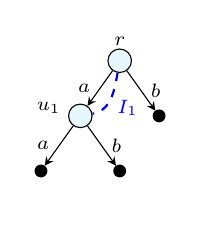
\begin{tikzpicture}
\tikzstyle{level 1}=[level distance=7mm,sibling distance = 10mm]
\tikzstyle{level 2}=[level distance=7mm,sibling distance=10mm]
\tikzstyle{level 3}=[level distance=7mm,sibling distance=15mm]
\tikzstyle{level 4}=[level distance=7mm,sibling distance=8mm]

%\draw [help lines, step=0.5] (-3,-3) grid (3,0);

\begin{scope}[->, >=stealth]
\node (0) [circ] {}
child{
  node (1) [circ] {}
  child{
    node (3) [term, label=below:{}] {}
    edge from parent node [left] {\scriptsize $a$}
  }
  child{
    node (4) [term,label=below:{}] {}
    edge from parent node [right] {\scriptsize $b$}
  }
  edge from parent node [left] {\scriptsize $a$}
}
child{
  node (2) [term, label=below:{}] {}
  edge from parent node [right] {\scriptsize $b$}
}
;
\end{scope}

\draw [dashed, thick, blue, in=10,out=-100] (0) to (1);



\node [black] at (0,0.25) {\scriptsize $r$};
\node [black] at (-.9,-0.6) {\scriptsize $u_1$};



\node [blue] at (.1,-.6) {\scriptsize $I_1$};

\end{tikzpicture}
\caption{$\Max$ with absentmindedness}
\label{fig-allexmp-absentm}
\end{subfigure}


%\end{center}
\caption{Recalls of $\Max$}
\label{fig:recall-examples}
\end{figure}
